\documentclass{article}
\usepackage{graphicx}
\usepackage[utf8]{inputenc}
\usepackage[T1]{fontenc}
\usepackage{makecell}
\usepackage{subfig}
\usepackage{diagbox}
\usepackage{needspace}
\usepackage{hyperref}
\usepackage{amsmath}
\usepackage[dvipsnames]{xcolor}
\usepackage[polish]{babel}
\usepackage[a4paper,
            left=1in,
            right=1in,
            top=1in,
            bottom=1in]{geometry}
\usepackage{selinput}
\usepackage{amsmath,amssymb}
\SelectInputMappings{
  cacute={ć},        
  lslash={ł}
}
\usepackage{listings}
\usepackage{color}
\usepackage{gensymb}

\definecolor{dkgreen}{rgb}{0,0.6,0}
\definecolor{gray}{rgb}{0.5,0.5,0.5}
\definecolor{mauve}{rgb}{0.58,0,0.82}

% \newcommand{\code}[1]{\textcolor{Fuchsia}{\textbf{\texttt{#1}}}}
\renewcommand{\contentsname}{Spis treści}
\addto\captionspolish{\renewcommand{\refname}{Źródła}}

\renewcommand*\descriptionlabel[1]{\hspace\leftmargin$#1$}
\addto\captionspolish{\renewcommand{\figurename}{Zdjęcie}}

\title{%
    Zadanie rekrutacyjne do KN Solvro\\
    \large{Sekcja uczenia maszynowego}
}
\author{Krzysztof Głowacz}
\date{wiosna 2025}

\makeatletter         
\def\@maketitle{
\raggedleft

\includegraphics[height = 15mm]{logo.png}\\[8ex]
\vspace{1.5cm}
\begin{center}
{\Huge \@title }\\[6ex]
{\Large  \@date}\\[15ex]
{\Large  \@author}\\[40ex]
\end{center}}
\makeatother

\lstset{frame=tb,
  language=Python,
  aboveskip=3mm,
  belowskip=3mm,
  showstringspaces=false,
  columns=flexible,
  basicstyle={\small\ttfamily},
  numbers=none,
  numberstyle=\tiny\color{gray},
  keywordstyle=\color{blue},
  commentstyle=\color{dkgreen},
  stringstyle=\color{mauve},
  breaklines=true,
  breakatwhitespace=true,
  tabsize=3
}

\definecolor{light-gray}{gray}{0.95}
\newcommand{\code}[1]{\colorbox{light-gray}{\texttt{#1}}}

\begin{document}

\maketitle
\tableofcontents
\clearpage

\section{Wstęp}
    W niniejszym raporcie przedstawione zostało rozwiązanie zadania rekrutacyjnego do sekcji uczenia maszynowego Koła Naukowego Solvro (rekrutacja wiosenna 2025). Zadanie polegało na eksploracyjnej analizie danych oraz klasteryzacji podanego zbioru \cite{instrukcja}.

\section{Analiza danych}
    Zbiór danych, pochodzący z bazy danych TheCocktailDB, zawierał listę koktajli wraz ze składnikami niezbędnymi do ich przyrządzenia. Link do zbioru danych został dołączony do sekcji Źródeł tego raportu \cite{zbior_danych}.

    W celu przeprowadzenia wstępnej analizy danych (\textit{EDA}) napisany został skrypt \code{src/eda.py}, który miał za zadanie:
    \begin{itemize}
        \item wczytać dane z pliku w formacie JSON do formatu DataFrame z biblioteki Pandas,
        \item wyświetlić podstawowe statystyki danych,
        \item wygenerować pełny raport opisujący dane korzystając z biblioteki ydata-profiling.
    \end{itemize}
    Na zdjęciu nr \ref{fig:run_eda} przedstawiony został fragment wyjścia standardowego po uruchomieniu skryptu.

    \begin{figure}[!htbp]%
        \centering
        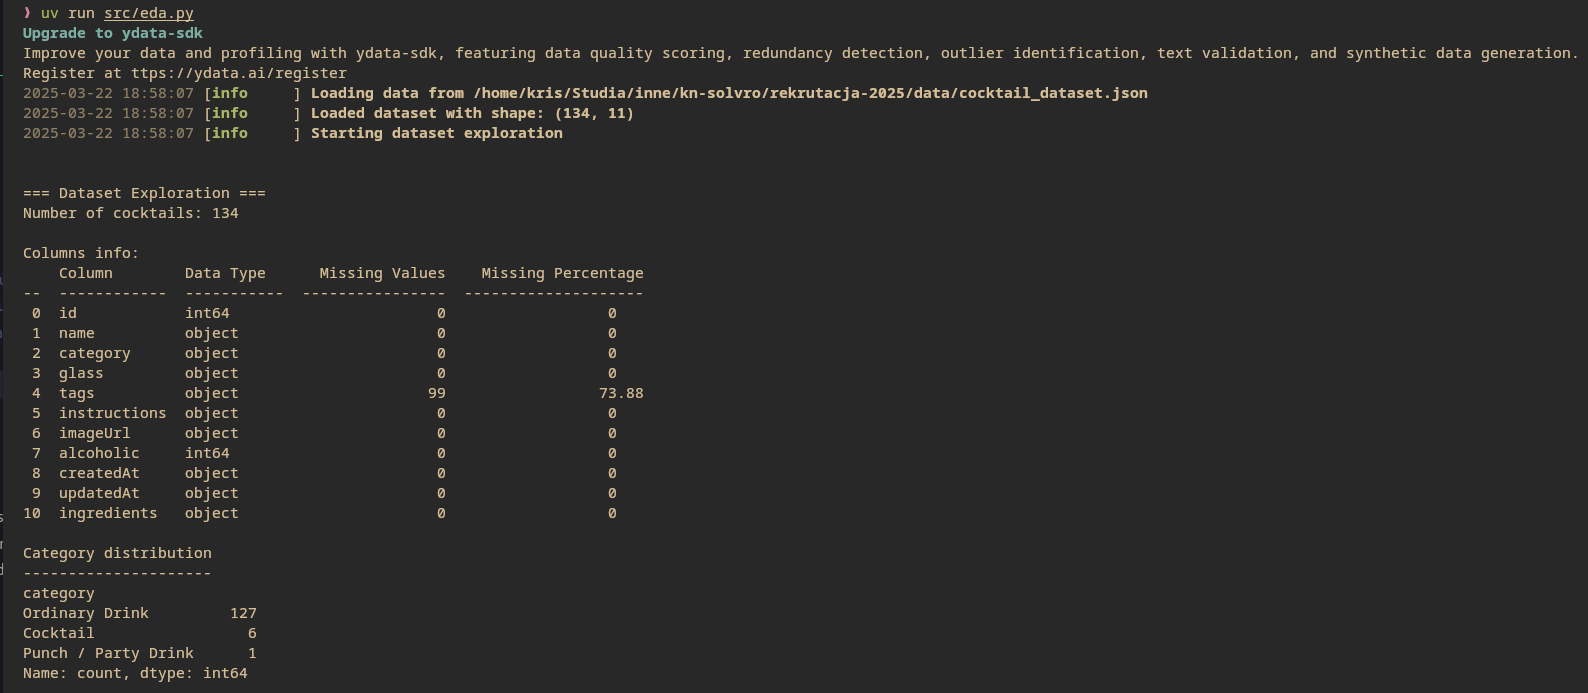
\includegraphics[width=\textwidth]{eda_run.png}
        \caption{Uruchomienie skryptu src/eda.py}%
        \label{fig:run_eda}
    \end{figure}

    Informacje dostarczone przez skrypt i wygenerowany raport pozwoliły na wyciągnięcie nastepujących wniosków:
    \begin{enumerate}
        \item Każdy koktajl ze zbioru danych opisany jest przez 11 cech, przy czym 4 z nich są zupełnie nieistotne z punktu widzenia dalszej analizy, ponieważ albo zawierają informacje typowo bazodanowe (kolumny: \textit{id}, \textit{createdAt}, \textit{updatedAt}), albo 
    \end{enumerate}


\section{Przygotowanie danych}
Przedmiotem analizy był zbiór Jester \cite{Jester}, który obejmował 100 różnych żartów wraz z ocenami ich śmieszności od niespełna 75 tysięcy osób. Żarty oceniane były w skali $(-10.0, 10.0)$. Przygotowanie danych wymagało w pierwszej części połączenia 3 plików z ocenami (po ok. 24 tys. ocen na każdy z plików), a następnie dla każdego wiersza wybranie wszystkich kolumn poza pierwszą (gdyż ta zawierała informację o liczbie ocenionych żartów przez danego użytkownika) i zamianę wartości \textit{99} na \code{NaN}, ponieważ oryginalny zbiór danych liczbą 99 sygnalizował brak oceny (\textit{null}), którego reprezentacją w bibliotece \textbf{numpy} jest właśnie \code{NaN}. Ostatecznie zbiór wszystkich ocen miał rozmiar: 73421 wierszy $\times$ 100 kolumn i prezentował się następująco (pierwsze 10. wierszy, kolumny symbolizują numery kolejnych żartów):

    \begin{table}[!htbp]%
        \centering
        \begin{tabular}{l|rrrrcrr}
             & 1 & 2 & 3 & 4 & $\dots$ & 99 & 100 \\ \hline
            0 & -7.82 & 8.79 & -9.66 & -8.16 & & NaN & NaN \\
            1 & 4.08 & -0.29 & 6.36 & 4.37 & & -4.32 & 1.07 \\
            2 & NaN & NaN & NaN & NaN & & NaN & NaN \\
            3 & NaN & 8.35 & NaN & NaN & & NaN & NaN \\
            4 & 8.50 & 4.61 & -4.17 & -5.39 & & 1.80 & 1.60 \\
            5 & -6.17 & -3.54 & 0.44 & -8.50 & & -5.05 & -3.45 \\
            6 & NaN & NaN & NaN & NaN & & NaN & NaN \\
            7 & 6.84 & 3.16 & 9.17 & -6.21 & & 1.31 & 0.00 \\
            8 & -3.79 & -3.54 & -9.42 & -6.89 & & -3.40 & -4.95 \\
            9 & 3.01 & 5.15 & 5.15 & 3.01 & & NaN & NaN \\
        \end{tabular}
        \caption{Przykładowe oceny śmieszności kolejnych żartów (od 10 osób)}
        \label{tab:example_ratings}
    \end{table}

\noindent Aby móc trenować model sieci neuronowej na zebranych danych konieczne było przypisanie jednej wartości dla każdego żartu, ponieważ celem modelu jest znalezienie takiej \textbf{funkcji}, która możliwie najlepiej opisze mapowanie treści żartu na poziom jego śmieszności. Funkcja natomiast z definicji jest takim przyporządkowaniem, które każdemu elementowi z jednego zbioru przyporządkowuje dokładnie jeden element z drugiego zbioru. Z tego powodu każdemu ze 100 żartów przypisana została średnia arytmetyczna z jego ocen. Otrzymano więc wektor długości 100, gdzie najmniejsza średnia ocen wyniosła: $-3.705$, a największa: $3.363$. Wektor ten stał się wektorem etykiet \code{Y}.

\vspace{0.2cm}

\noindent W celu przygotowania wektora tekstów \code{X} połączono sto plików w formacie \textit{html}, z których każdy zawierał tekst danego żartu. Przy użyciu biblioteki \textbf{beautifulsoup4} pobrane zostały treści żartów, które po dodatkowym przetworzeniu (usunięciu znaków białych, usunięciu prefiksów ,,Q.'' oraz ,,A.'' dla żartów z pytaniem i odpowiedzią, itp.) trafiły do jednej listy. Finalnie pierwsze pięć elementów listy wyglądało następująco:

    \begin{enumerate}
        \item A man visits the doctor. The doctor says "I have bad news for you.You have cancer and Alzheimer's disease". The man replies "Well, thank God I don't have cancer!"
        \item This couple had an excellent relationship going until one day he came home from work to find his girlfriend packing. He asked her why she was leaving him and she...
        \item What's 200 feet long and has 4 teeth?  The front row at a Willie Nelson Concert.
        \item What's the difference between a man and a toilet?  A toilet doesn't follow you around after you use it.
        \item What's O. J. Simpson's Internet address?  Slash, slash, backslash, slash, slash, escape.
    \end{enumerate}

\noindent Tak przygotowane teksty żartów należało następnie poddać procesowi wektoryzacji opartemu o tzw. słownik. Każda treść żartu przekształcona została na wektor $x \in \mathbb{N}^{D}$, który na i-tej pozycji zawierał liczbę wystąpień słowa/sylaby o indeksie i. Podczas laboratorium przetestowano dwa modele przetwarzania języka naturalnego: \textbf{Bert (bert-base-cased)} oraz \textbf{FastText}. W przypadku tego pierwszego długość wektora $x$ równa była 768, a w przypadku drugiego 300. Tak przekształcona lista żartów stała się wektorem \code{X}.

\vspace{0.2cm}

\noindent Ostatnim etapem przygotowania danych był podział wektorów \code{X} i \code{Y} na zbiór danych uczących i walidacyjnych. W tym celu skorzystano z funkcji \code{train\_test\_split} z biblioteki \textbf{sklearn.model\_selection}. Ze względu na stosunkowo niewielki rozmiar zbioru danych wejściowych dokonano podziału w stosunku 3:7, tj. rozmiar zbioru danych testowych stanowił 30\% rozmiaru zbioru wszystkich danych. Aby zapewnić powtarzalność całego procesu między kolejnymi jego wykonaniami wszystkie funkcje mogące zachowywać się w sposób pseudolosowy otrzymywały taki sam generator liczb pseudolosowych (z takim samym ziarnem).

\section{Wykorzystanie modelu MLP}
    \textit{Multi-layer Perceptron (MLP)} jest algorytmem uczenia nadzorowanego, który poszukuje funkcji
    $$f: \mathbb{R}^{m} \rightarrow \mathbb{R}^{o}$$
    ($m$ - liczba wymiarów wejściowych, $o$ - liczba wymiarów wyjściowych) poprzez trening na zbiorze danych uczących. Może zostać użyty w przypadku problemu regresji, a także klasyfikacji. Pomiędzy warstwami wejściową i wyjściową może znajdować się jedna lub więcej warstw, zwanych warstwami ukrytymi. Symboliczna reprezentacja sieci tego typu pochodząca z dokumentacji użytej biblioteki \cite{scikit} zaprezentowana jest na poniższym zdjęciu:
    \begin{figure}[!htbp]%
        \centering
        % \includegraphics[width=7cm]{multilayerperceptron_network.png}
        \caption{Przykładowa sieć MLP z jedną warstwą ukrytą}%
        \label{fig:mlp_example}
    \end{figure}

    \noindent W dalej opisanych eksperymentach używany był model \code{MLPRegressor}, którego najważniejsze hiperparametry (z punktu widzenia tego laboratorium) to:

    \begin{enumerate}
        \item \textbf{hidden\_layer\_sizes} - tablica, której i-ty element reprezentuje liczbę neuronów w i-tej warstwie ukrytej. We wszystkich testach używana była jedna warstwa ukryta. Domyślna wartość: \textit{(100,)}.
        \item \textbf{solver} - metoda optymalizacji wag. W testach używana była wartość \textit{sgd}, która używa stochastyczny gradient do wyznaczenia kierunku poszukiwań. Domyślna wartość: \textit{adam}.
        \item \textbf{alpha} - siła regularyzacji L2. W testach używaną wartością było $0.0$. Domyślna wartość: $0.0001$.
        \item \textbf{learning\_rate} - strategia aktualizacji tempa uczenia. W testach ustawiona była wartość \textit{constant}, która oznacza stałą prędkość uczenia parametryzowaną przez \textbf{learning\_rate\_init}. Domyślna wartość: \textit{constant}.
        \item \textbf{learning\_rate\_init} - początkowa prędkość uczenia, kontroluje wielkość ,,kroku'' przy aktualizacji wag. Domyślna wartość: $0.001$.
        \item \textbf{random\_state} - określa generator pseudolosowy używany przy niektórych wartościach, np. wagach. W testach używano \code{np.random.RandomState(42)} w celu zapewnienia powtarzalności między kolejnymi wykonaniami danego testu. Domyślna wartość: \textit{None}.
        \item \textbf{warm\_start} - w przypadku ustawienia flagi \code{True} poprzednie rozwiązanie jest używane ponowne przy inicjalizacji następnego (w przeciwnym przypadku poprzednie rozwiązanie jest usuwane). W testach flaga była ustawiona na wartość \code{True}. Domyślna wartość: \code{False}.
        \item \textbf{max\_iter} - maksymalna liczba iteracji. W przypadku użycia metody \textit{sgd} wartość ta określa liczbę epok. W testach ustawiona była wartość $1$, ponieważ liczba epok kontrolowana była w inny sposób (przez zewnętrzny licznik), który umożliwiał łatwe tworzenie wykresów. Domyślna wartość: \textit{200}.
    \end{enumerate}
    
    \subsection{Model MLP o domyślnej konfiguracji}
        Etap testowania wpływu poszczególnych hiperparametrów na jakość działania sieci neuronowej typu MLP rozpoczynał się od sprawdzenia działania podstawowego modelu o domyślnej konfiguracji. Kod odpowiedzialny za przygotowanie takiego podstawowego modelu wyglądał następująco:
\begin{lstlisting}
rng = np.random.RandomState(42)

mlp = MLPRegressor(solver='sgd', alpha=0.0, learning_rate='constant', random_state=rng, warm_start=True, max_iter=1)
\end{lstlisting}

    \noindent Wykresy na poniższych zdjęciach przedstawiają wartość funkcji kosztu (błąd średniokwadratowy) odpowiednio zbioru treningowego i walidacyjnego w zależności od epoki:
        % \begin{figure}[!htbp]%
        %     \centering
        %     \subfloat[\centering Model \textbf{Bert}]{{\includegraphics[width=7cm]{charts/bert_default.png} }}%
        %     \qquad
        %     \subfloat[\centering Model \textbf{FastText}]{{\includegraphics[width=7cm]{charts/fasttext_default.png} }}%
        %     \caption{Porównanie funkcji kosztu w zależności od epoki dla obu zbiorów, dla obu modeli NLP}
        %     \label{default_comparison}
        % \end{figure}

    \noindent Wykres dla modelu Bert świadczy o tym, że po ok. 500 epokach pojawiło się zjawisko \textit{overfittingu} - model MLP zaczął się zbyt dobrze dopasowywać do danych treningowych, na co wskazują rosnące wartości MSE dla zbioru walidacyjnego - model zaczął sobie gorzej radzić z predykowaniem wartości dla nieznanych próbek, ponieważ przeuczył się na danych treningowych. Wykres dla modelu FastText z kolei nie wykazuje oznak \textit{overfittingu}, ale generalnie widoczne jest bardzo małe dopasowanie do danych w przypadku obu zbiorów, a drobne różnice między wartościami MSE dla zbioru uczącego i walidacyjnego mogą wynikać z natury samych zbiorów - dane testowe mogą zawierać przykładowo więcej szumów i trudniejszych tekstów do predykowania.

\vspace{1cm}
\hrulefill
\bibliographystyle{plain}
\bibliography{references}
\end{document}
